% Created 2023-01-25 mié 16:30
% Intended LaTeX compiler: pdflatex
\documentclass[aspectratio=169, usenames,svgnames,dvipsnames]{beamer}
\usepackage[utf8]{inputenc}
\usepackage[T1]{fontenc}
\usepackage{graphicx}
\usepackage{longtable}
\usepackage{wrapfig}
\usepackage{rotating}
\usepackage[normalem]{ulem}
\usepackage{amsmath}
\usepackage{amssymb}
\usepackage{capt-of}
\usepackage{hyperref}
\usepackage{color}
\usepackage{listings}
\usepackage{mathpazo}
\usepackage{gensymb}
\usepackage{amsmath}
\usepackage{diffcoeff}
\usepackage{steinmetz}
\usepackage{mathtools}
\bibliographystyle{plain}
\usepackage{siunitx}
\sisetup{output-decimal-marker={,}}
\DeclareSIUnit{\watthour}{Wh}
\hypersetup{colorlinks=true, linkcolor=Blue, urlcolor=Blue}
\renewcommand{\thefootnote}{\fnsymbol{footnote}}
\newcommand{\laplace}[1]{\mathbf{#1}(\mathbf{s})}
\newcommand{\slp}{\mathbf{s}}
\newcommand{\fasor}[1]{\mathbf{#1}(\omega)}
\newcommand{\atan}{\mathrm{atan}}
\parskip=5pt
\usetheme{Boadilla}
\usecolortheme{rose}
\usefonttheme{serif}
\author{Oscar Perpiñán Lamigueiro}
\date{}
\title{Teoremas Generales}
\subtitle{Teoría de Circuitos II}
\setbeamercolor{alerted text}{fg=blue!50!black} \setbeamerfont{alerted text}{series=\bfseries}
\AtBeginSubsection[]{\begin{frame}[plain]\tableofcontents[currentsubsection,sectionstyle=show/shaded,subsectionstyle=show/shaded/hide]\end{frame}}
\AtBeginSection[]{\begin{frame}[plain]\tableofcontents[currentsection,hideallsubsections]\end{frame}}
\beamertemplatenavigationsymbolsempty
\setbeamertemplate{footline}[frame number]
\setbeamertemplate{itemize items}[triangle]
\setbeamertemplate{enumerate items}[circle]
\setbeamertemplate{section in toc}[circle]
\setbeamertemplate{subsection in toc}[circle]
\hypersetup{
 pdfauthor={Oscar Perpiñán Lamigueiro},
 pdftitle={Teoremas Generales},
 pdfkeywords={},
 pdfsubject={},
 pdfcreator={Emacs 28.2 (Org mode 9.6)}, 
 pdflang={Spanish}}
\begin{document}

\maketitle

\section{Teoremas de linealidad}
\label{sec:orge2ae583}

\begin{frame}[label={sec:orgc2a5f66}]{Elementos lineales}
\begin{itemize}
\item Un circuito eléctrico es lineal si los elementos pasivos y activos que incluye son lineales.
\item Un \alert{elemento pasivo} es lineal si la relación entre la tensión entre sus terminales y la corriente que lo recorre es lineal: \alert{resistencias, condensadores y bobinas}.
\item Una \alert{fuente dependiente} es lineal si su salida (tensión o corriente) tiene una relación lineal con la magnitud del circuito de la que depende.
\item Un circuito lineal tiene dos propiedades:
\begin{itemize}
\item Homogeneidad o \alert{proporcionalidad}.
\item Aditividad o \alert{superposición}.
\end{itemize}
\end{itemize}
\end{frame}

\begin{frame}[label={sec:org8313837}]{Homogeneidad o Proporcionalidad}
Sea \(y(t)\) la respuesta de un \alert{circuito lineal} a una excitación \(x(t)\). 

Si la excitación es multiplicada por una \alert{constante}, \(K \cdot x(t)\), la respuesta del circuito será modificada por la misma constante, \(K \cdot y(t)\).

\begin{center}
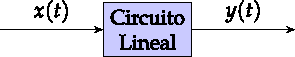
\includegraphics[width=0.6\textwidth]{../figs/proporcionalidad.pdf}
\end{center}
\end{frame}

\begin{frame}[label={sec:org34de0f9}]{Teorema de superposición}
\begin{columns}
\begin{column}{0.5\columnwidth}
La respuesta de un \alert{circuito lineal} a varias fuentes de excitación actuando simultáneamente es igual a la suma de las respuestas que se tendrían cuando actuase cada una de ellas por separado

\[
y(t) = \sum_i y_i(t)
\]
\end{column}

\begin{column}{0.5\columnwidth}
\begin{center}
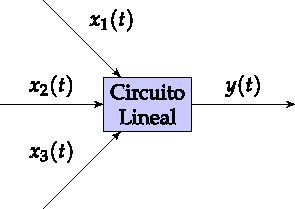
\includegraphics[width=.9\linewidth]{../figs/superposicion.pdf}
\end{center}
\end{column}
\end{columns}
\end{frame}

\begin{frame}[label={sec:orgfdeaad0}]{Análisis de un circuito mediante superposición}
\begin{block}{Procedimiento}
\begin{enumerate}
\item Se apagan todas las fuentes \alert{independientes} del circuito menos una.
\begin{itemize}
\item Las fuentes de tensión se sustituyen por un cortocircuito (\(U = 0\)).
\item Las fuentes de corriente se sustituyen por un circuito abierto (\(I = 0\)).
\item Las fuentes \alert{dependientes} \alert{no} se modifican.
\end{itemize}
\item Se analiza el circuito, obteniendo la respuesta individual a la fuente que permanece activa.
\item Se repite este procedimiento para cada una de las fuentes \alert{independientes} del circuito.
\item La respuesta total del circuito es la suma de las respuestas individuales.
\end{enumerate}
\end{block}
\end{frame}

\begin{frame}[label={sec:orgf20f933}]{Análisis de un circuito mediante superposición}
\begin{block}{Observaciones}
\begin{itemize}
\item \alert{Siempre} hay que aplicar este método cuando en un circuito conviven fuentes de \alert{diferente frecuencia} (o fuentes de corriente continua y corriente alterna).
\item En el caso de fuentes de corriente alterna \alert{sinusoidal}, la respuesta debe expresarse en el \alert{dominio del tiempo}. \alert{No} se pueden \alert{sumar} los \alert{fasores} que corresponden a \alert{frecuencias diferentes}.
\item En el primer paso del procedimiento, se pueden agrupar las fuentes que funcionan a la misma frecuencia y calcular la respuesta del circuito en esa frecuencia.
\end{itemize}
\end{block}
\end{frame}

\begin{frame}[label={sec:orge742781}]{Cálculo de potencia con superposición}
El principio de superposición aplica a tensiones y corrientes, pero \alert{no} a potencias. Supongamos \(i(t) = i_1(t) + i_2(t)\):
\begin{align*}
  p(t) &= R \cdot i^2(t) =\\
       &= R \cdot (i_1(t) + i_2(t))^2 =\\
       &=R \cdot (i_1^2(t) + i_2^2(t) + 2\cdot i_1(t) \cdot i_2(t))\\
  p(t) &\neq p_1(t) + p_2(t)
\end{align*}
\end{frame}
\begin{frame}[label={sec:orgce9bf36}]{Cálculo de potencia con superposición}
\begin{itemize}
\item Cuando las señales son \alert{ortogonales en un período}\footnote{Dos señales son ortogonales si cumplen la siguiente ecuación: \[<f_1, f_2>_T = \int_T f_1(t) \cdot f_2(t) dt = 0\]} se pueden sumar las potencias \alert{medias} de cada circuito.
\end{itemize}
\begin{align*}
  P = \sum_i P_i
\end{align*}
\begin{itemize}
\item Ejemplos de señales ortogonales: sinusoidales con diferente frecuencia, una sinusoide con una continua, \ldots{}
\end{itemize}
\end{frame}


\section{Teoremas de reciprocidad y sustitución}
\label{sec:orge706758}

\begin{frame}[label={sec:org2356174}]{Teorema de reciprocidad}
La matriz de impedancias de un circuito pasivo es simétrica. En
consecuencia, al intercambiar la posición de una fuente de tensión, la
corriente de cortocircuito en la otra rama no cambia.

\begin{center}
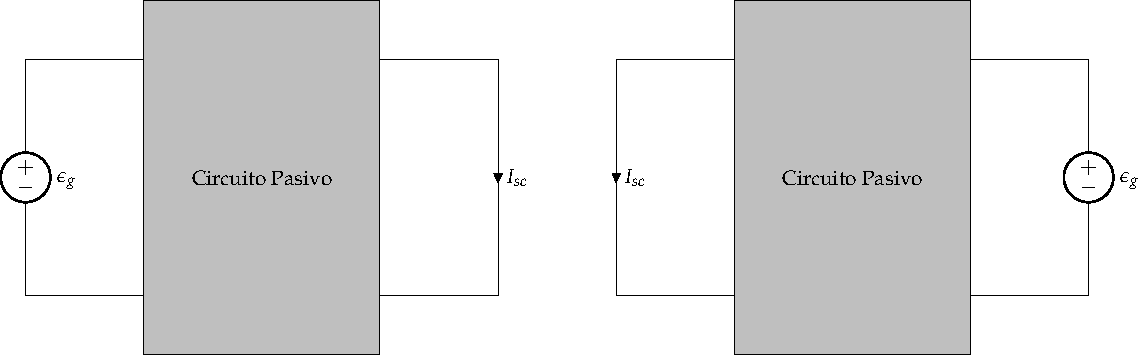
\includegraphics[width=.9\linewidth]{../figs/TeoremaReciprocidadTension.pdf}
\end{center}
\end{frame}

\begin{frame}[label={sec:orgb0ba823}]{Teorema de reciprocidad}
La matriz de admitancias de un circuito pasivo es simétrica. En
consecuencia, al intercambiar la posición de una fuente de corriente, la
tensión de circuito abierto en la otra posición no cambia.

\begin{center}
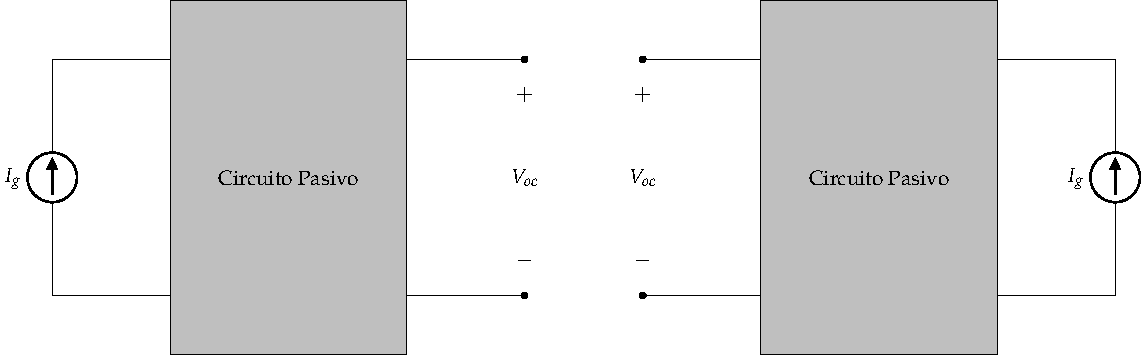
\includegraphics[width=.9\linewidth]{../figs/TeoremaReciprocidadCorriente.pdf}
\end{center}
\end{frame}

\begin{frame}[label={sec:org8dbb2d4}]{Teorema de sustitución}
\begin{center}
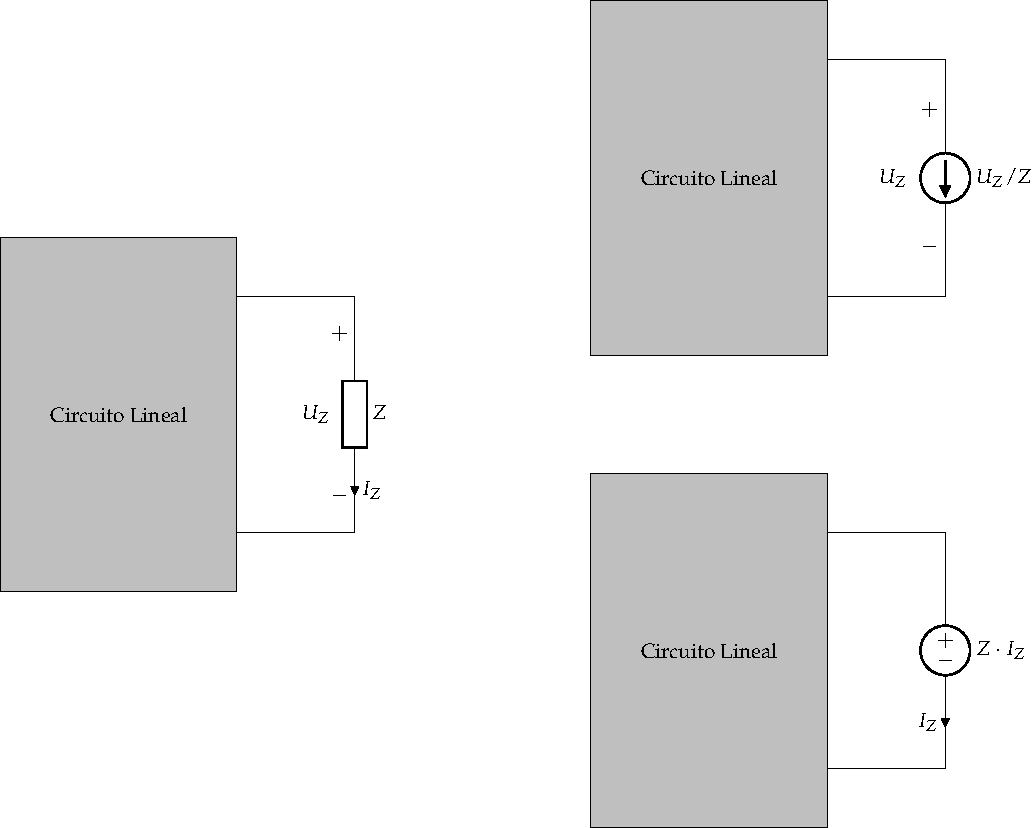
\includegraphics[height=0.9\textheight]{../figs/TeoremaSustitucion.pdf}
\end{center}
\end{frame}

\section{Teorema de compensación}
\label{sec:org1a65bd3}

\begin{frame}[label={sec:org9206e5d}]{Planteamiento}
¿Cuál es la variación en la respuesta \(I_k\) debida a una variación en la impedancia \(Z\)?

\begin{center}
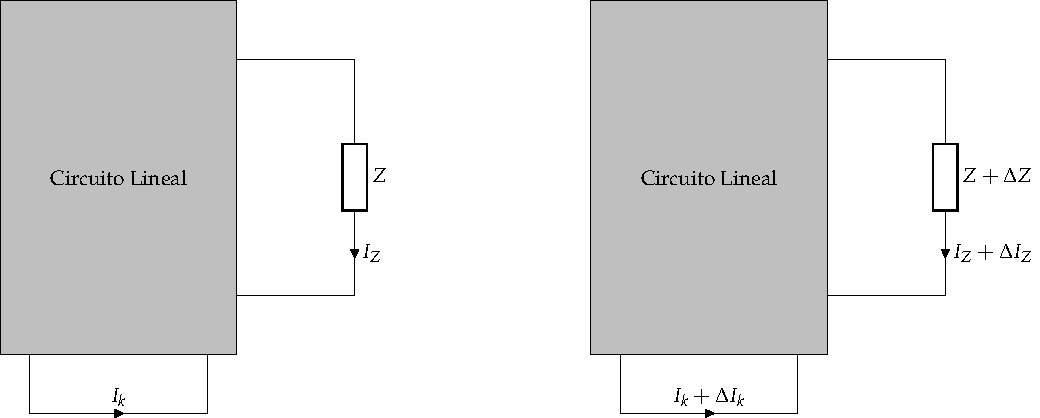
\includegraphics[width=0.95\textwidth]{../figs/TeoremaCompensacion0.pdf}
\end{center}
\end{frame}


\begin{frame}[label={sec:orgdac1bd7}]{Aplicamos teorema de sustitución}
\begin{center}
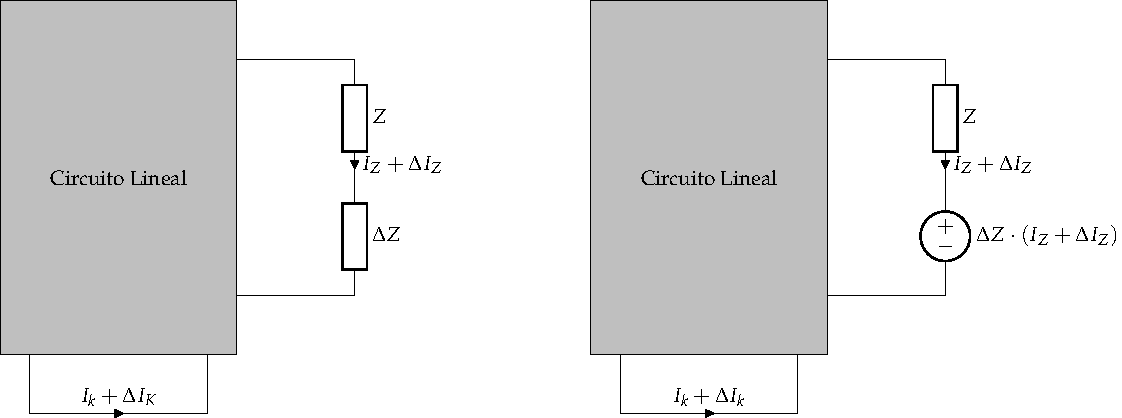
\includegraphics[width=0.95\textwidth]{../figs/TeoremaCompensacion1.pdf}
\end{center}
\end{frame}

\begin{frame}[label={sec:org820a34f}]{A continuación, teorema de superposición}
\begin{center}
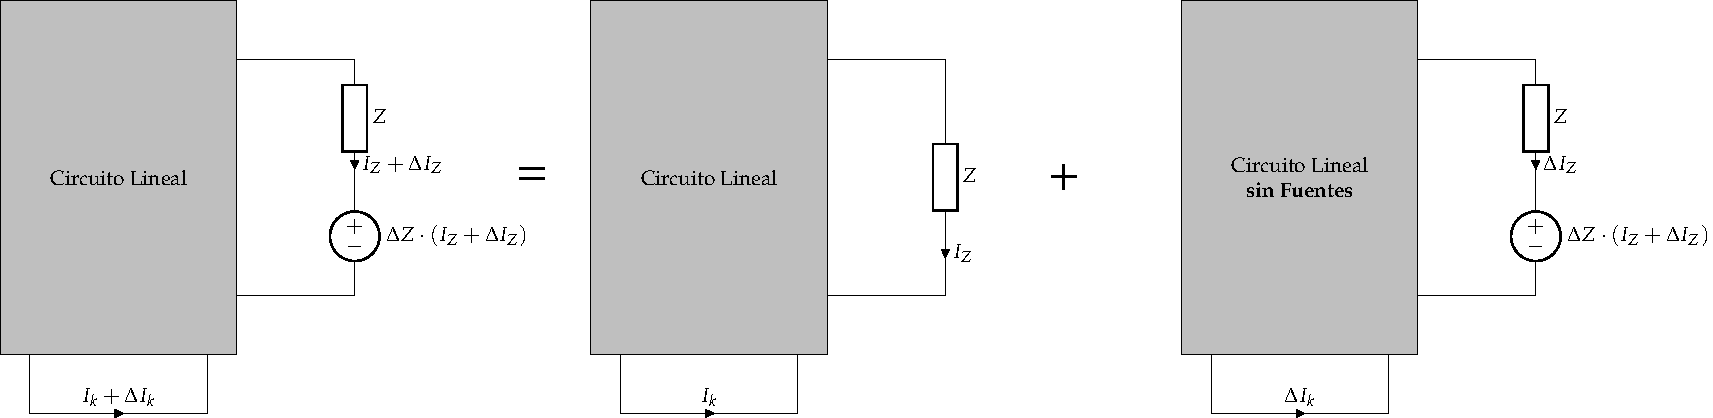
\includegraphics[width=0.95\textwidth]{../figs/TeoremaCompensacion2.pdf}
\end{center}
\end{frame}

\begin{frame}[label={sec:org4314070}]{Nuevamente, teorema de sustitución}
En el último circuito, expresamos la fuente como:

\[
  \Delta Z \cdot (I_Z + \Delta I_Z) = \Delta Z \cdot I_Z + \Delta Z \cdot \Delta I_Z
\]

El último sumando representa la tensión en la impedancia \(\Delta Z\) recorrida por la corriente de la rama, \(\Delta I_z\). Esta observación nos permite volver a utilizar el teorema de sustitución.


\begin{center}
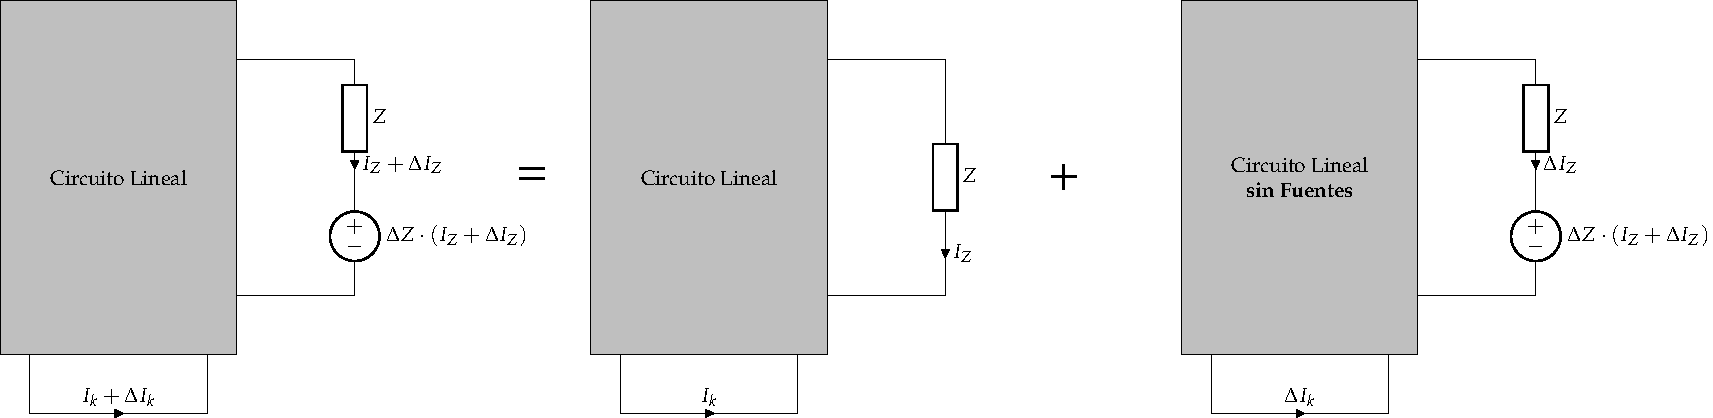
\includegraphics[width=0.95\textwidth]{../figs/TeoremaCompensacion2.pdf}
\end{center}
\end{frame}

\begin{frame}[label={sec:org228544c}]{Solución}
Para determinar el cambio en la respuesta, \(\Delta I_k\), debido a una variación en la impedancia, \(\Delta Z\):

\begin{enumerate}
\item Se calcula la corriente \(I_z\) en el circuito original.
\item Se apagan las fuentes independientes y se sustituye la impedancia \(Z\) por una impedancia de valor \(Z + \Delta Z\) en serie con una fuente de tensión de valor \(\Delta Z \cdot I_z\).
\item En el circuito resultante se calcula la respuesta, \(\Delta I_k\).
\end{enumerate}

\begin{center}
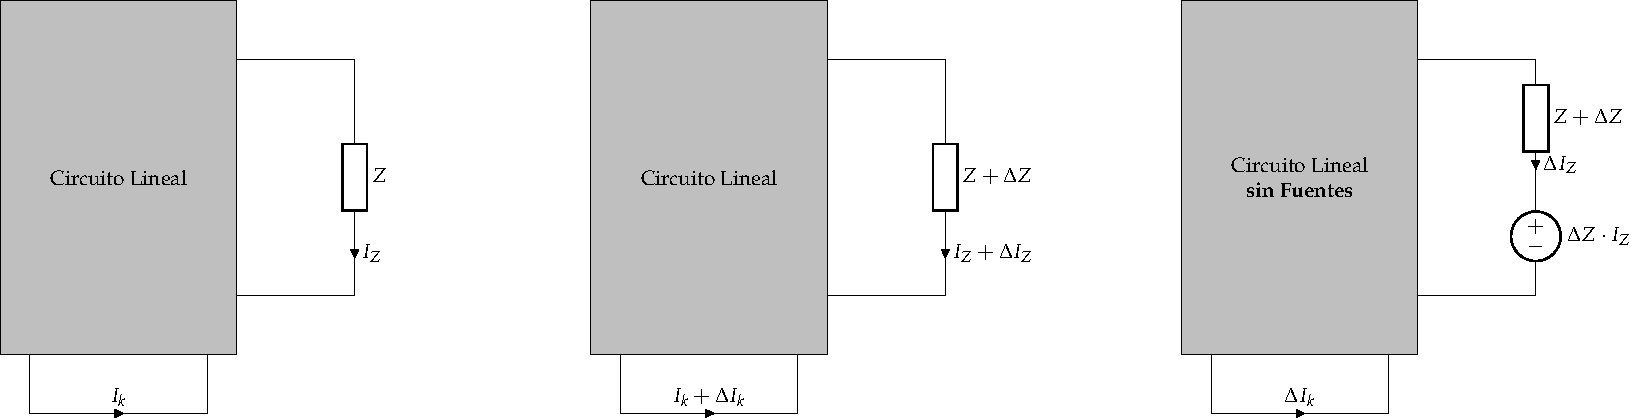
\includegraphics[height=0.45\textheight]{../figs/TeoremaCompensacion.pdf}
\end{center}
\end{frame}


\section{Teorema de Millman}
\label{sec:org1d5df63}

\begin{frame}[label={sec:org3b398c1}]{Planteamiento}
El Teorema de Millman permite resolver la tensión entre dos puntos A y O, siendo éste un punto común de un conjunto de impedancias, y siendo conocidas las tensiones con el punto A y las impedancias.

\begin{center}
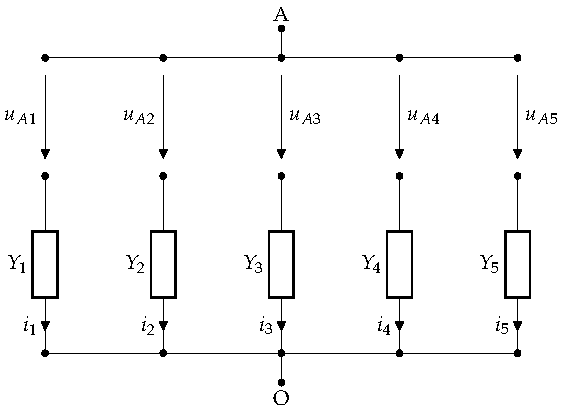
\includegraphics[height=0.7\textheight]{../figs/Millman.pdf}
\end{center}
\end{frame}

\begin{frame}[label={sec:org7ed9c08}]{Resolución}
La tensión \(u_{AO}\) es:
\[
  u_{AO} = u_{Aj} + i_j/Y_j
\]

Despejando \(i_j\):

\[
  i_j = Y_j \cdot (u_{AO} - u_{Aj})
\]

En el nudo O se puede plantear LKC:

\[
  \sum_{j = 1}^n i_j = 0
\]

Por tanto:
\[
  \sum_{j = 1}^n Y_j \cdot (u_{AO} - u_{Aj}) = 0 \rightarrow \boxed{u_{AO} = \frac{\sum_{j = 1}^n Y_j u_{Aj}}{\sum_{i = 1}^n Y_j}}
\]
\end{frame}

\begin{frame}[label={sec:org6c45f72}]{Aplicación}
Este teorema permite resolver rápidamente circuitos como el siguiente:

\begin{center}
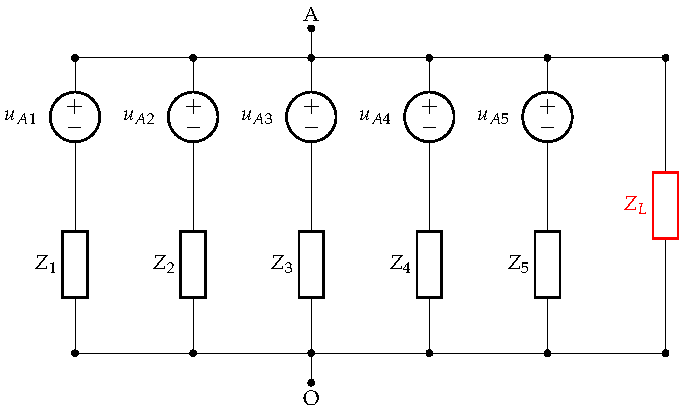
\includegraphics[height=0.6\textheight]{../figs/Millman_aplicacion.pdf}
\end{center}

\[
  u_{AO} = \frac{\sum_{j = 1}^n u_{Aj}/Z_j}{{\color{red} 1/Z_L} + \sum_{i = 1}^n 1/Z_j}
\]
\end{frame}

\section{Teorema de Rosen}
\label{sec:org1b141d1}

\begin{frame}[label={sec:org26ad519}]{Planteamiento}
Una estrella se puede transformar en un polígono (pero no al revés si \(n > 3\)):
\begin{columns}
\begin{column}{0.5\columnwidth}
\begin{center}
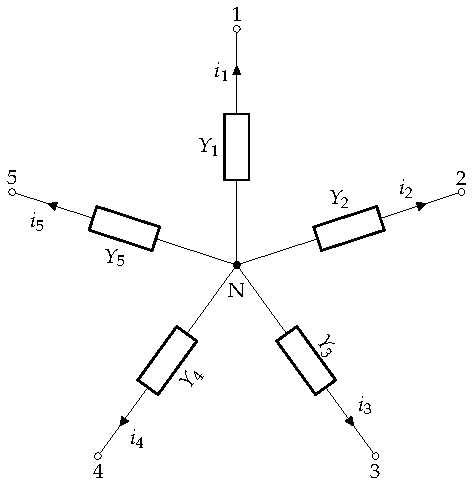
\includegraphics[width=0.9\textwidth]{../figs/Rosen_Y.pdf}
\end{center}
\end{column}

\begin{column}{0.5\columnwidth}
\begin{center}
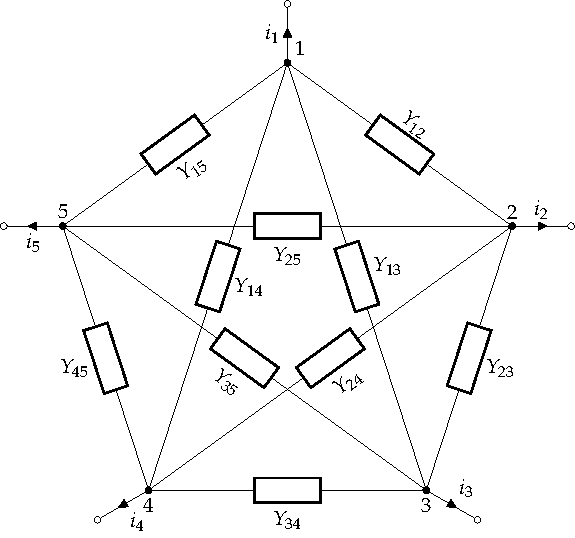
\includegraphics[width=0.9\textwidth]{../figs/Rosen_D.pdf}
\end{center}
\end{column}
\end{columns}
\end{frame}


\begin{frame}[label={sec:org67129ec}]{Corrientes en el polígono}
\begin{columns}
\begin{column}{0.5\columnwidth}
\begin{center}
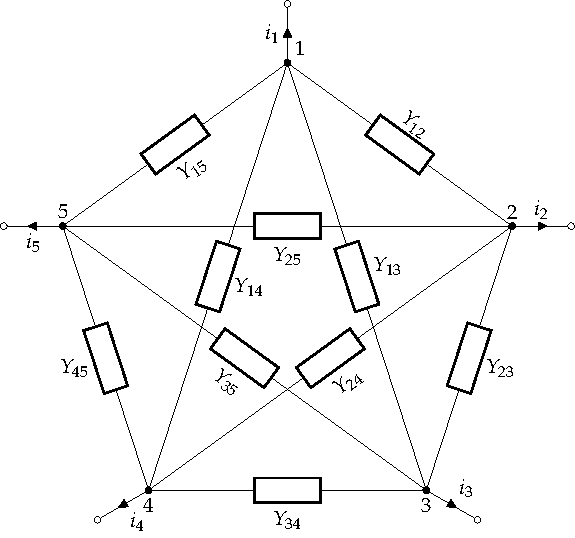
\includegraphics[width=0.9\textwidth]{../figs/Rosen_D.pdf}
\end{center}
\end{column}

\begin{column}{0.5\columnwidth}
Podemos calcular la corriente que sale por cada terminal:
\[
  i_j = \sum_{\substack{k = 1\\k \neq j}}^n i_{kj} = \sum_{\substack{k = 1\\k \neq j}}^n u_{kj} \cdot Y_{kj} = \sum_{k = 1}^n u_{kj} \cdot Y_{kj}  
\]
teniendo en cuenta que \(u_{kk} = 0\).
\end{column}
\end{columns}
\end{frame}

\begin{frame}[label={sec:org39adcaf}]{Corrientes en la estrella}
\begin{columns}
\begin{column}{0.5\columnwidth}
\begin{center}
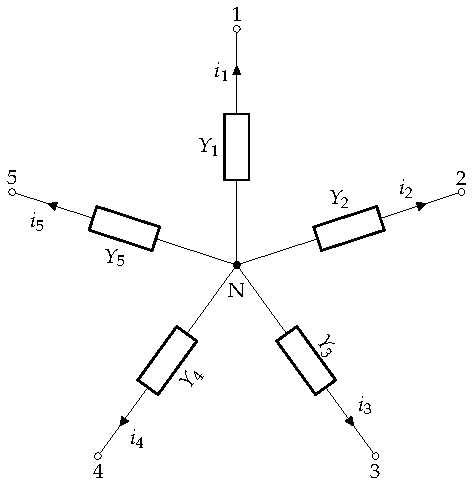
\includegraphics[width=0.9\textwidth]{../figs/Rosen_Y.pdf}
\end{center}
\end{column}

\begin{column}{0.5\columnwidth}
La corriente en cada rama es:
\[
  i_j = Y_j \cdot u_{jN}
\]
La tensión \(u_{jN}\) se puede calcular con el Teorema de Millman:

\[
  u_{jN} = \frac{\sum_{k = 1}^n u_{kj} Y_k}{\sum_{k  = 1}^n Y_k}
\]

Por tanto:
\[
  i_j = Y_j \cdot \frac{\sum_{k = 1}^n u_{kj} Y_k}{\sum_{k  = 1}^n Y_k}
\]
\end{column}
\end{columns}
\end{frame}

\begin{frame}[label={sec:org8837ce2}]{Resolución}
Para que los dos circuitos sean equivalentes, las ecuaciones de las corrientes deben dar el mismo resultado:

\[
  \frac{\sum_{k = 1}^n u_{kj} Y_k Y_j}{\sum_{k  = 1}^n Y_k} = \sum_{k = 1}^n u_{kj} \cdot Y_{kj}  
\]
Denominando \(Y_Y = \sum_{k  = 1}^n Y_k\) y agrupando dentro del sumatorio:
\[
  \sum_{k = 1}^n u_{kj} \frac{Y_k Y_j}{Y_Y} = \sum_{k = 1}^n u_{kj} \cdot Y_{kj}  
\]

Por tanto:

\[
  \boxed{Y_{kj} = \frac{Y_k Y_j}{\sum_{k  = 1}^n Y_k}}
\]
\end{frame}

\begin{frame}[label={sec:org693f2b0}]{Aplicación}
\begin{itemize}
\item Ejemplo para \(n = 3\) (estrella \(\rightarrow\) triángulo)
\end{itemize}

\begin{columns}
\begin{column}{0.3\columnwidth}
\begin{center}
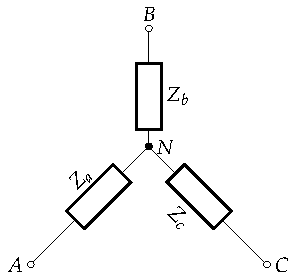
\includegraphics[height=0.5\textheight]{../figs/Impedancia_Estrella.pdf}
\end{center}
\end{column}

\begin{column}{0.3\columnwidth}
\[
  \boxed{Y_{kj} = \frac{Y_k Y_j}{\sum_{k  = 1}^n Y_k}}
\]

\begin{align*}
  Y_{ab} &= \frac{Y_a Y_b}{Y_a + Y_b + Y_c}\\
  \\
  Y_{bc} &= \frac{Y_b Y_c}{Y_a + Y_b + Y_c}\\
  \\
  Y_{ca} &= \frac{Y_c Y_a}{Y_a + Y_b + Y_c}\\
\end{align*}
\end{column}
\begin{column}{0.3\columnwidth}
\begin{center}
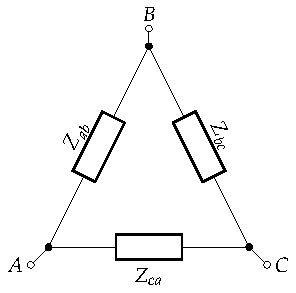
\includegraphics[height=0.5\textheight]{../figs/Impedancia_Triangulo.pdf}
\end{center}
\end{column}
\end{columns}
\end{frame}

\section{Teoremas de Thévenin/Norton}
\label{sec:orged0d2f9}

\begin{frame}[label={sec:org147492a}]{Teoremas de Thévenin/Norton}
\framesubtitle{Thévenin}

Cualquier \alert{red lineal} compuesta por elementos activos y pasivos puede sustituirse, desde el punto de vista de sus terminales externos AB, por una \alert{fuente de tensión} (generador de Thévenin, \(\epsilon_{th}\)) en \alert{serie} con una impedancia (impedancia de Thévenin, \(Z_{th}\)).

\begin{center}
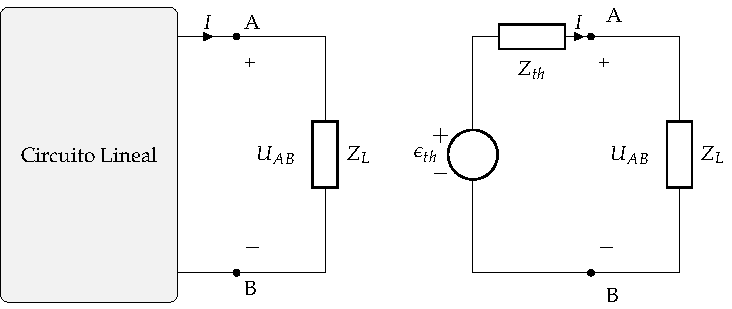
\includegraphics[height=0.6\textheight]{../figs/EquivalenteThevenin.pdf}
\end{center}
\end{frame}

\begin{frame}[label={sec:org309f167}]{Teoremas de Thévenin/Norton}
\framesubtitle{Norton}
Cualquier \alert{red lineal} compuesta por elementos activos y pasivos puede sustituirse, desde el punto de vista de sus terminales externos AB, por una \alert{fuente de corriente} (generador de Norton, \(I_N\)) en \alert{paralelo} con una impedancia (impedancia de Norton, \(Z_N\)).

\begin{center}
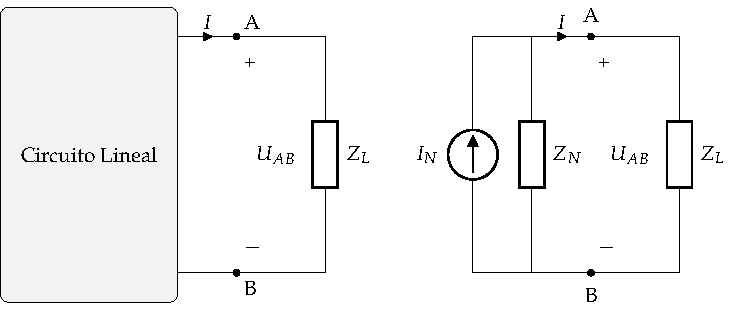
\includegraphics[height=0.6\textheight]{../figs/EquivalenteNorton.pdf}
\end{center}
\end{frame}

\begin{frame}[label={sec:org366d5b0}]{Teoremas de Thévenin/Norton}
\framesubtitle{Cálculo del equivalente de Thévenin}
\begin{center}
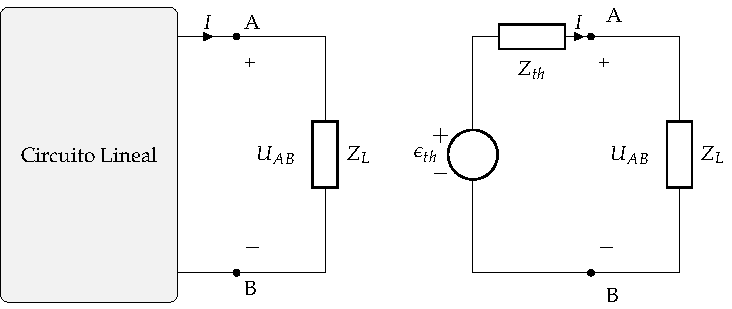
\includegraphics[height=0.38\textheight]{../figs/EquivalenteThevenin.pdf}
\end{center}

\begin{itemize}
\item Circuito Abierto (\(Z_L \to \infty, \quad U_{AB} = U_{oc}\))
\end{itemize}
\[
\boxed{\epsilon_{th} = U_{oc}}
\]
\begin{itemize}
\item Cortocircuito (\(Z_L = 0, \quad I = I_{sc}\))
\end{itemize}
\[
\boxed{Z_{th} = \frac{\epsilon_{th}}{I_{sc}} = \frac{U_{oc}}{I_{sc}}}
\]
\end{frame}

\begin{frame}[label={sec:org5267d2e}]{Teoremas de Thévenin/Norton}
\framesubtitle{Cálculo del equivalente de Norton}
\begin{center}
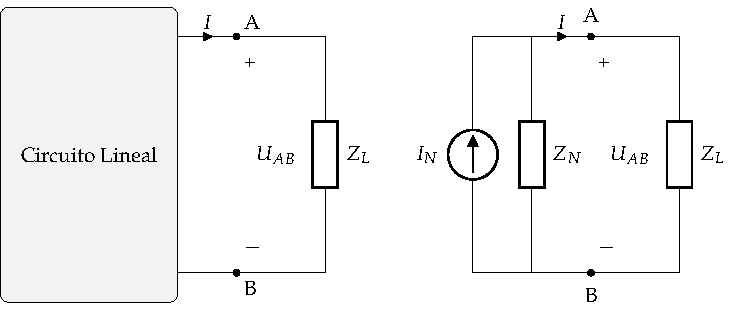
\includegraphics[height=0.38\textheight]{../figs/EquivalenteNorton.pdf}
\end{center}

\begin{itemize}
\item Cortocircuito (\(Z_L = 0, \quad I = I_{sc}\))
\end{itemize}
\[
\boxed{I_N = I_{sc}}
\]
\begin{itemize}
\item Circuito Abierto (\(Z_L \to \infty, \quad U_{AB} = U_{oc}\))
\end{itemize}
\[
\boxed{Z_N = \frac{U_{oc}}{I_N} = \frac{U_{oc}}{I_{sc}}}
\]
\end{frame}

\begin{frame}[label={sec:org70ae911}]{Teoremas de Thévenin/Norton}
\framesubtitle{Cálculo de Thévenin/Norton}

\begin{block}{Observaciones}
\begin{itemize}
\item Cálculo de la impedancia:
\begin{itemize}
\item Si el circuito \alert{no} contiene fuentes dependientes, se puede realizar \alert{apagando} todos los \alert{generadores} y obteniendo la impedancia equivalente.
\item Si el circuito contiene fuentes dependientes, es necesario conectar un \alert{generador de prueba} a la salida del circuito y obtener la relación entre la tensión y corriente de este generador.
\end{itemize}

\item Gracias a la equivalencia de fuentes, una vez obtenido uno de los equivalentes se puede obtener el otro mediante una transformación.
\end{itemize}
\end{block}
\end{frame}

\begin{frame}[label={sec:org8bb3410}]{Máxima Transferencia de Potencia}
\framesubtitle{Planteamiento}
Sea el circuito lineal de la figura. ¿Qué impedancia \(Z_L\) hay que conectar en los terminales AB para que el circuito entregue la máxima potencia disponible?

\begin{center}
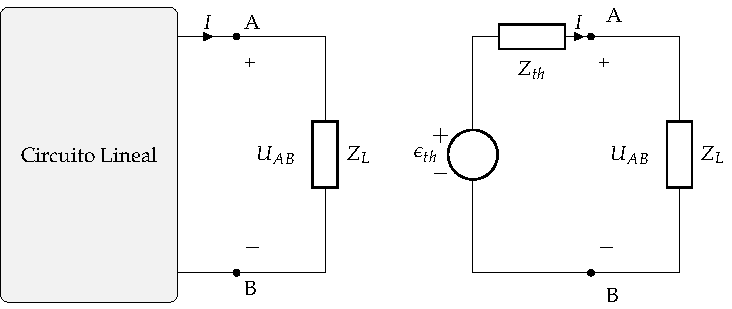
\includegraphics[height=0.55\textheight]{../figs/EquivalenteThevenin.pdf}
\end{center}

Resolvemos esta pregunta mediante el generador equivalente de Thévenin.
\end{frame}



\begin{frame}[label={sec:org9286556}]{Máxima Transferencia de Potencia}
\framesubtitle{Ecuaciones}
Calculamos la potencia activa en la impedancia de carga \(Z_L\):
\begin{columns}
\begin{column}{0.3\columnwidth}
\begin{center}
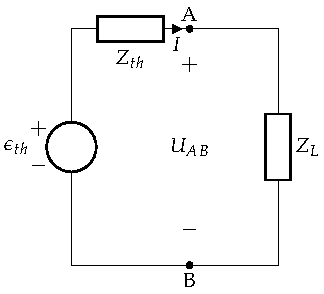
\includegraphics[height=0.45\textheight]{../figs/EquivalenteThevenin0.pdf}
\end{center}
\end{column}

\begin{column}{0.2\columnwidth}
\begin{align*}
  \overline{Z}_{th} &= R_{th} + jX_{th}\\
  \overline{Z}_L &= R_L + jX_L\\
\end{align*}
\end{column}

\begin{column}{0.4\columnwidth}
\begin{align*}
\overline{I} &= \frac{\overline{\epsilon}_{th}}{\overline{Z}_{th} + \overline{Z}_L}\\
P_L &= I^2 \cdot R_L\\
\Aboxed{P_L &= \frac{\epsilon^2_{th}}{|\overline{Z}_{th} + \overline{Z}_L|^2} \cdot R_L}
\end{align*}
\end{column}
\end{columns}

Las condiciones de máximo son: 
\[
  \boxed{%
    \diffp{P_L}{X_L} = 0 \quad%
    \diffp{P_L}{R_L} = 0%
  }
\]
\end{frame}

\begin{frame}[label={sec:orgf9430e0}]{Máxima Transferencia de Potencia}
\framesubtitle{Reactancia}
A partir de la expresión de potencia en la carga\ldots{}
\[
  P_L = \frac{\epsilon^2_{th}}{|\overline{Z}_{th} + \overline{Z}_L|^2} \cdot R_L
\]
calculamos la derivada parcial respecto de la reactancia:
\[
  \diffp{P_L}{X_L} = \epsilon^2_{th} \cdot R_L \cdot \left[\frac{-1}{\left((R_L + R_{th})^2 + (X_L + X_{th})^2\right)^2} \cdot 2 \cdot (X_L + X_{th})\right]
\]
Aplicamos la condición de máximo y obtenemos un resultado parcial:
\[
   \diffp{P_L}{X_L} = 0 \Rightarrow \boxed{X_L = - X_{th}}
\]
\end{frame}

\begin{frame}[label={sec:org82e198f}]{Máxima Transferencia de Potencia}
\framesubtitle{Resistencia}
Simplificamos la expresión de la potencia teniendo en cuenta el resultado anterior (\(X_L = - X_{th}\)):
\[
  P_L = \frac{\epsilon^2_{th}}{(R_{th} + R_L)^2} \cdot R_L
\]
Calculamos la derivada parcial respecto de la resistencia:
\begin{align*}
  \diffp{P_L}{R_L} &= \epsilon^2_{th} \cdot \left[\frac{1}{(R_L + R_{th})^2} - 2 \cdot \frac{R_L}{(R_L + R_{th})^3}\right]\\
		   &= \frac{\epsilon^2_{th} \cdot (R_{th} - R_L)}{(R_L + R_{th})^3}
\end{align*}
Nuevamente, aplicamos la condición de máximo y obtenemos la resistencia:
\[
   \diffp{P_L}{R_L} = 0 \Rightarrow \boxed{R_L = R_{th}}
\]
\end{frame}

\begin{frame}[label={sec:org8499b26}]{Máxima Transferencia de Potencia}
\framesubtitle{Impedancia de carga}

Dado un circuito lineal (del que podemos calcular su equivalente de Thévenin) \ldots{}
\begin{center}
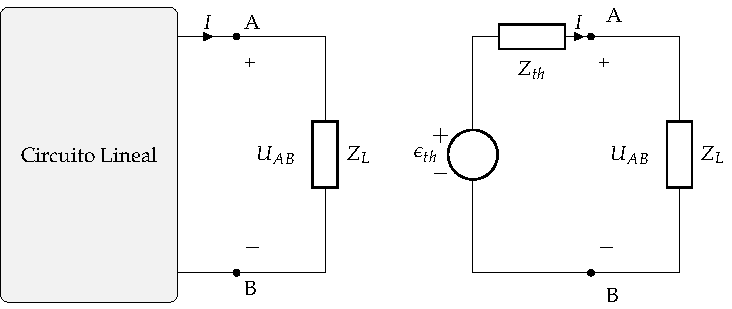
\includegraphics[height=0.45\textheight]{../figs/EquivalenteThevenin.pdf}
\end{center}

\ldots{} la impedancia de carga que hay que conectar entre sus terminales AB para obtener la máxima potencia disponible es:
\[
  \boxed{\overline{Z}_L = \overline{Z}_{th}^*}
\]
\end{frame}

\begin{frame}[label={sec:orgb0c93a7}]{Máxima Transferencia de Potencia}
\framesubtitle{Máxima potencia disponible}

La máxima potencia disponible en la carga es:
\begin{center}
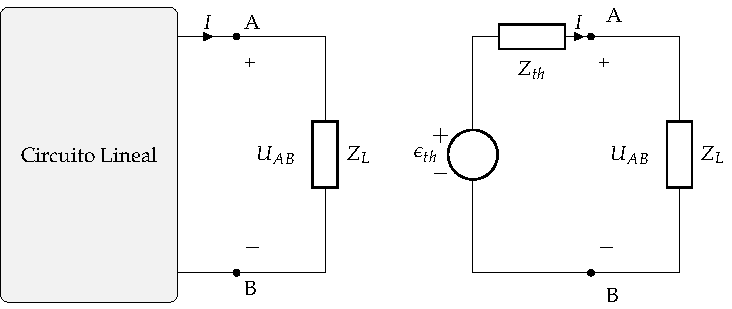
\includegraphics[height=0.45\textheight]{../figs/EquivalenteThevenin.pdf}
\end{center}

\begin{equation*}
  \left.
    \begin{matrix}
      \overline{Z}_L = \overline{Z}_{th}^*\\
      P_L = \frac{\epsilon^2_{th}}{|\overline{Z}_{th} + \overline{Z}_L|^2} \cdot R_L
    \end{matrix} \right\}\rightarrow
  \boxed{P_L = \frac{\epsilon^2_{th}}{4 R_{th}}}
\end{equation*}
\end{frame}



\section{Teorema de Everitt}
\label{sec:org9786618}

\begin{frame}[label={sec:orgfa1e016}]{Planteamiento}
Si a la entrada de un circuito no disipativo (LC) existe adaptación de impedancias, a la salida de este circuito también hay adaptación. Dado que \(\overline{Z}_L \neq \overline{Z}^*_g\), el circuito LC es una red adaptadora.

\begin{center}
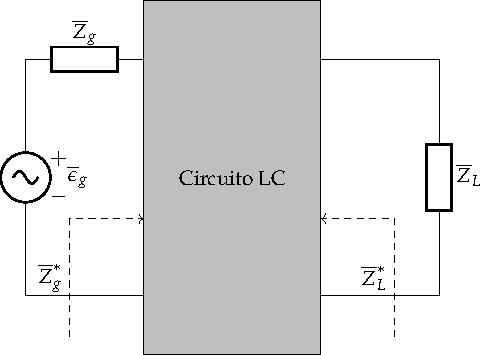
\includegraphics[height=0.7\textheight]{../figs/Everitt.pdf}
\end{center}
\end{frame}

\begin{frame}[label={sec:orgd4c672c}]{Potencia}
Dado que el circuito LC no consume potencia activa, la potencia a la entrada es la potencia consumida por la carga. Por tanto, si la potencia a la entrada es máxima (adaptación en la entrada), también lo será a la salida (adaptación a la salida).

\begin{center}
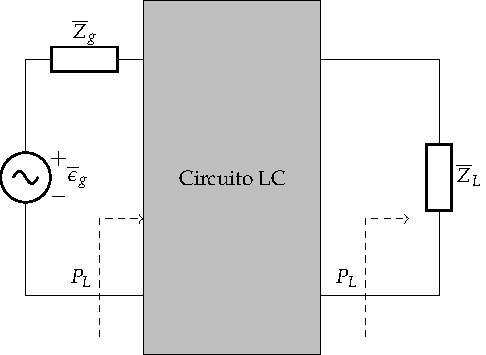
\includegraphics[height=0.7\textheight]{../figs/Everitt_potencia.pdf}
\end{center}
\end{frame}

\begin{frame}[label={sec:org4bcc1b2}]{Redes en cascada}
Si en una cascada de circuitos LC existe adaptación de impedancias en un punto de la cadena, existirá adaptación en cualquier punto de la misma.

\begin{center}
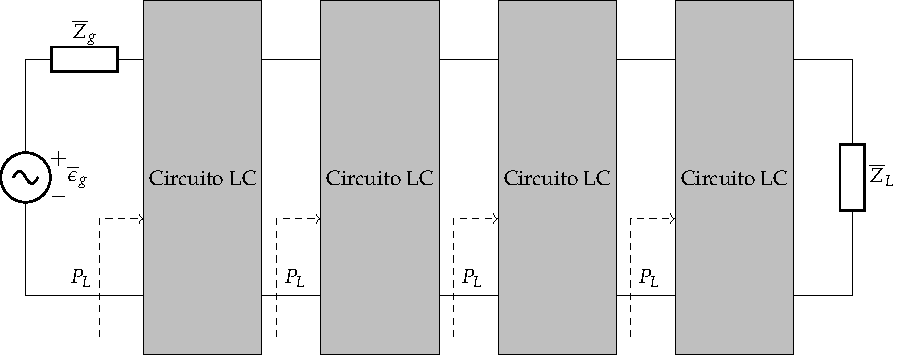
\includegraphics[height=0.7\textheight]{../figs/Everitt_cascada.pdf}
\end{center}
\end{frame}


\begin{frame}[label={sec:orgdef63ef}]{Diseño de redes adaptadoras}
Emplearemos redes en L compuestas por dos elementos reactivos.

\begin{center}
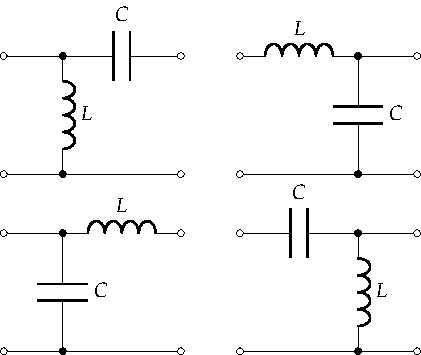
\includegraphics[height=0.7\textheight]{../figs/Everitt_LC.pdf}
\end{center}

Esta adaptación es selectiva: si varía la frecuencia, no habrá adaptación.
\end{frame}

\begin{frame}[label={sec:orgb8347cf}]{Diseño de redes adaptadoras}
La red debe diseñarse con el elemento paralelo en el extremo de la impedancia que tenga parte real mayor.

\begin{columns}
\begin{column}{0.5\columnwidth}
\begin{center}
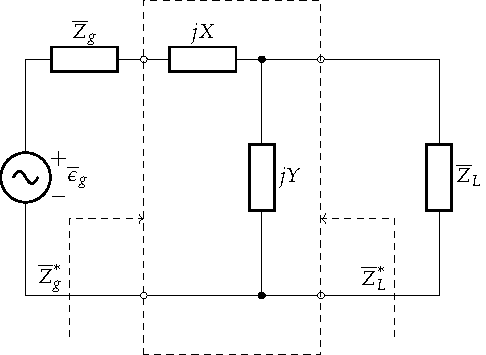
\includegraphics[width=\textwidth]{../figs/Everitt_XY1.pdf}
\end{center}
\end{column}


\begin{column}{0.5\columnwidth}
\begin{center}
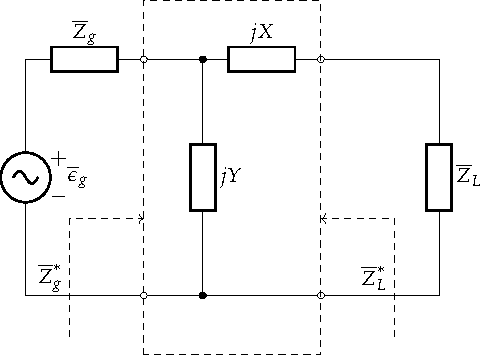
\includegraphics[width=\textwidth]{../figs/Everitt_XY2.pdf}
\end{center}
\end{column}
\end{columns}
\end{frame}

\begin{frame}[label={sec:org2059e28}]{Diseño de redes adaptadoras: \(R_g > R_L\)}
\begin{columns}
\begin{column}{0.3\columnwidth}
Condición:
\[
  \overline{Z}^*_L = jX + (jY || \overline{Z}_g) 
\]
Ecuaciones:
\begin{align*}
  R_L &= \Re\left(\frac{jY \cdot \overline{Z}_g}{jY + \overline{Z}_g}\right)\\
  X_L &= -X - \Im\left(\frac{jY \cdot \overline{Z}_g}{jY + \overline{Z}_g}\right)
\end{align*}
\end{column}

\begin{column}{0.7\columnwidth}
\begin{center}
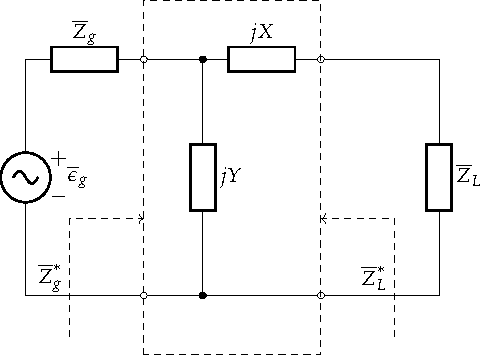
\includegraphics[height=0.8\textheight]{../figs/Everitt_XY2.pdf}
\end{center}
\end{column}
\end{columns}
\end{frame}

\begin{frame}[label={sec:org241c18d}]{Diseño de redes adaptadoras: \(R_L > R_g\)}
\begin{columns}
\begin{column}{0.3\columnwidth}
Condición:
\[
  \overline{Z}^*_g = jX + (jY || \overline{Z}_L) 
\]
Ecuaciones:
\begin{align*}
  R_g &= \Re\left(\frac{jY \cdot \overline{Z}_L}{jY + \overline{Z}_L}\right)\\
  X_g &= -X - \Im\left(\frac{jY \cdot \overline{Z}_L}{jY + \overline{Z}_L}\right)
\end{align*}
\end{column}

\begin{column}{0.7\columnwidth}
\begin{center}
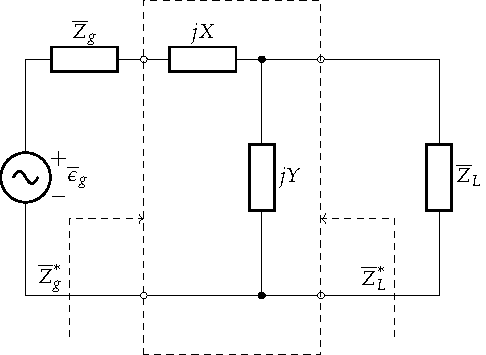
\includegraphics[height=0.8\textheight]{../figs/Everitt_XY1.pdf}
\end{center}
\end{column}
\end{columns}
\end{frame}

\begin{frame}[label={sec:org2edf2b2}]{Pérdidas de transmisión e inserción}
\begin{block}{Decibelio: potencias}
El \alert{decibelio} (\(\si{\decibel}\)) se emplea para medir la ganancia de potencia o la ratio de dos niveles de potencia:

\[
G_{dB} = 10 \log G = 10 \log \frac{P_2}{P_1}
\]
\begin{center}
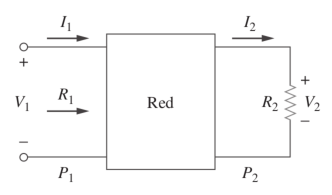
\includegraphics[height=0.5\textheight]{../figs/Red_Ganancia.pdf}
\end{center}
\end{block}
\end{frame}

\begin{frame}[label={sec:org9f43e52}]{Pérdidas de transmisión e inserción}
\begin{block}{Decibelio: tensiones}
Suponiendo \(R_1 = R_2\), también se emplea para medir la ganancia de tensión/corriente:

\[
G_{dB} = 10 \log \frac{U_2^2}{U_1^2} = 20 \log \frac{U_2}{U_1}
\]
\begin{center}
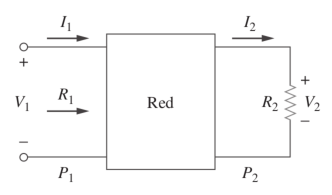
\includegraphics[height=0.5\textheight]{../figs/Red_Ganancia.pdf}
\end{center}
\end{block}
\end{frame}

\begin{frame}[label={sec:org5e78b68}]{Pérdidas de transmisión}
Las pérdidas de transmisión, \(\alpha_T\), asociadas a una red miden la relación entre la potencia de entrada, \(P_{in}\), y la potencia de salida, \(P_{out}\).


\begin{columns}
\begin{column}{0.7\columnwidth}
\begin{center}
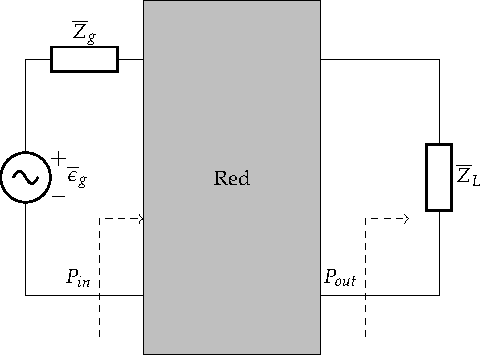
\includegraphics[height=0.6\textheight]{../figs/PerdidasTransmision.pdf}
\end{center}
\end{column}

\begin{column}{0.3\columnwidth}
\[
  \alpha_T = 10 \log \frac{P_{in}}{P_{out}} \unit{\decibel}
\]
\end{column}
\end{columns}

\begin{center}
Si la red es no disipativa (LC), \(P_{in} = P_{out} \rightarrow \alpha_T = \qty{0}{\decibel}\).
\end{center}
\end{frame}

\begin{frame}[label={sec:orgb63e6ac}]{Pérdidas de inserción}
Las pérdidas de inserción, \(\alpha_I\), asociadas a una red miden la relación entre la potencia entregada a la carga sin la red, \(P_L\), y la potencia entregada a la carga con la red insertada.

\[
  \alpha_I = 10 \log \frac{P_L}{P_{out}} \unit{\decibel}
\]

\begin{center}
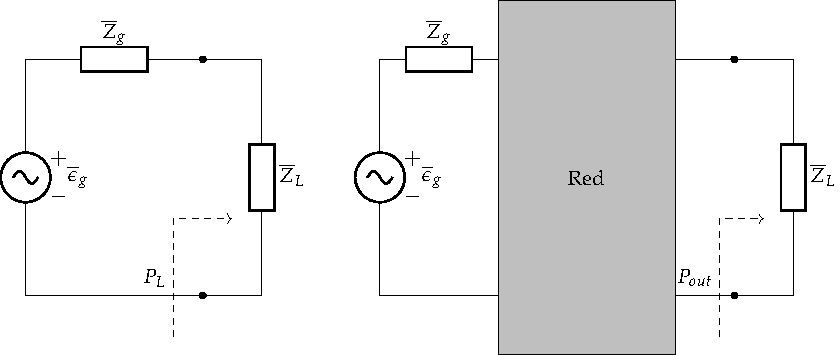
\includegraphics[height=0.45\textheight]{../figs/PerdidasInsercion.pdf}
\end{center}

En el caso de una red adaptadora, \(P_{out} > P_L\), por lo que \(\alpha_I < 0\) (ganancia de inserción).
\end{frame}
\end{document}